\chapter{High Mass Searches}
\label{ch:highMassSearches}
\section{Introduction}
The Standard Model (SM) of particle physics, which describes the electroweak interactions, consists of a Higgs-like scalar particle responsible for the generation of the masses of fundamental particles.
The discovery of a Higgs-like boson with a mass of approximately 125 $\textrm{GeV}$ by the ATLAS and CMS Collaborations confirmed the existence of this scalar particle in the SM.
However, the possibility of additional resonances at higher masses still exists.
This has been predicted by several popular models beyond the SM, such as the general two-Higgs-doublet models or models in which the SM Higgs boson mixes with a heavy electroweak singlet. Hence, the search for high-mass scalar bosons is a crucial aspect of the study of electroweak interactions.
In this paper, we focus on the search for an SM-like Higgs boson at high mass, decaying to a pair of Z bosons.
The focus is on the semi-leptonic channel, with the analysis being performed in the mass range from 500 $\textrm{GeV}$ to 3 $\textrm{TeV}$. Below 500 GeV, the Z+jet background dominates which kills the sensitivity at low scalar mass.
The data used for this analysis were recorded by the CMS experiment at the LHC in Run-2, with an integrated luminosity of 139 fb$^{-1}$ at a centre-of-mass energy of 13 $\textrm{TeV}$.
A new strategy called ``particle net" (PN) has been implemented to improve the identification of boosted hadronic Z jets, resulting in more accurate signal identification. This strategy helps in differentiating between QCD jets and Z-jets.
Two model-independent signal interpretations have been used in this analysis, both of which consider a charge-neutral heavy scalar boson with a mass above the SM Higgs boson mass. The narrow width approximation (NWA) interpretation assumes a negligible line width of the heavy boson.
The non-zero width assumption (NZWA) parametrized the width of the scalar boson as a function of its mass, allowing for a more general width assumption.
% The results of this analysis show no significant excess of events with respect to the standard model expectation.
Limits have been set on the product of the cross section for a new scalar boson and the branching fraction for its decay to ZZ for a large range of masses and widths.
The paper is structured as follows: In Section 2, we provide a brief description of the CMS detector, while Section 3 outlines the dataset used in the analysis and the Monte Carlo simulation. In Section 4, we explain the Matrix Element techniques employed in our analysis. The event selection, reconstruction, and PN strategy used in the analysis are described in Section 5. Section 6 provides a comprehensive explanation of the signal and background parametrization. Systematic uncertainties are discussed in Section 7, while Section 8 presents the results of the analysis. Finally, in Section 9, we provide a summary of our findings.
% figures/HighMassSearches

\section{Dataset and monte carlo simulation}
\label{sec:MC}

The dataset used in this analysis corresponds to proton-proton collisions recorded by the CMS detector during Run-2 with an integrated luminosity of 138 fb$^{-1}$ at a centre-of-mass energy of 13 TeV.
The data were collected between 2016 and 2018 and were used to search for a new scalar resonance in the mass range from 500 GeV to 3 TeV.
The data were processed using the CMS software framework, which includes a set of reconstruction algorithms and software tools for event selection, data analysis, and data storage.
The CMS detector and the dataset used in this analysis provide a powerful tool for the search for new physics beyond the SM, and the high luminosity of Run-2 dataset provides improved sensitivity to new physics phenomena.

Signal events with SM-like couplings are generated at next-to-leading order (NLO) in quantum chromodynamics (QCD) with \POWHEG\ 2.0~\cite{Frixione:2007vw,Bagnaschi:2011tu,Nason:2009ai,Nason:2004rx,Alioli:2010xd} for the gluon-gluon fusion (ggF) and vector boson fusion (VBF) production modes. The $\PX \to \cPZ\cPZ \to 2\ell2\cPq$ decay is modeled with \textsc{JHUGen}\ 7.0.2~\cite{Gao:2010qx,Bolognesi:2012mm,Anderson:2013afp,Gritsan:2016hjl}, including corrections for the $\cPZ\cPZ$ branching fraction and the angular correlation among the fermions. A wide range of masses $m_{\PX}$ from 500 GeV to 3 TeV is generated with the width $\Gamma_{\PX}$ set according to the SM Higgs boson expectation for $m_{\PX}$ up to 1 TeV. For higher masses, the width $\Gamma_{\PX} = 0.5m_{\PX}$ is chosen, which approximately corresponds to the SM Higgs boson prediction for $m_{\PX} = 1$ TeV. The generated samples are used to derive a generic signal parameterization.

While NLO accuracy in QCD is used in production, no modelling of the interference with the background is included at this stage of the simulation. The MELA matrix element package~\cite{Gao:2010qx,Bolognesi:2012mm,Anderson:2013afp,Gritsan:2016hjl}, based on \textsc{JHUGen} for both $\PH(125)$ and $\PX$ signal, and on \MCFM\ 7.0~\cite{MCFM,Campbell:2011bn,Campbell:2013una} for the continuum background, allows modelling of interference of a broad $\PX$ resonance with SM background in either ggF or electroweak (EW) production, the latter including VBF and $\PV\PH$ processes.

The background from the production of two $\cPZ$ bosons from quark-antiquark annihilation, $\cPq\overline{\cPq} \to \cPZ\cPZ/ \cPZ\gamma^*\to \ff$, is evaluated at NLO with \POWHEG~\cite{Nason:2013ydw} and \MGvATNLO 2.3.2~\cite{MadGraph}. The $\PW\cPZ$ production is generated at LO with \PYTHIA\ 8.212~\cite{Sjostrand:2008za}, normalized to NNLO in QCD accuracy~\cite{Grazzini:2016swo}. The $\cPZ + \text{jets}$ ($\cPZ\to\ell^+\ell^-$) simulation is a composite sample comprising a set of exclusive LO samples with various associated parton multiplicities, including a dedicated sample with associated $\cPqb$-quark production. These samples are produced at LO with \MGvATNLO and corrected to NLO QCD accuracy with a K factor depending on the $\pt$ of the dilepton pair, derived from \MGvATNLO simulation at NLO with FxFx merging scheme~\cite{Frederix:2012ps}. The simulation of top quark-antiquark pair production, $\ttbar$, is performed with \POWHEG{} at NLO in QCD~\cite{Frixione:2007nw}.

All generated samples are interfaced with \PYTHIA, configured with the CUETP8M1 tune~\cite{CUETP8M1} for the simulation of parton showers, hadronization, and underlying event effects. All simulated events are further processed with a \GEANTfour{} based description~\cite{Agostinelli2003250} of the CMS detector and reconstructed with the same algorithms used for data. Supplementary minimum bias (pileup) interactions are added to the simulated events with a multiplicity determined to match that observed in the data.

\section{Matrix element techniques}
The Matrix Element (ME) method is widely used in particle physics to model the behaviour of particle interactions and decays.
These techniques use the information about the underlying dynamics of a process, encoded in the matrix element, to provide a robust and precise estimation of signal and background contributions.
It provides an alternative to traditional methods of separating signal and background events, such as cuts on kinematic observables or multivariate classifiers.
By using the information encoded in the matrix elements, they allow for full exploitation of all available information and provide more accurate modelling of the physics process under study.


In this study, the ME method is employed in three distinct ways. Firstly, it is used to apply weights to generated events from various models, reducing the need for a full simulation of the samples. Secondly, the ME method is utilized to create a comprehensive model of a broad high-mass resonance $\PX$, including its interference with the Standard Model (SM) background, for use in the likelihood fit. Finally, the ME method is applied to create optimal discriminants for categorizing events based on their production mechanism or to separate the signal from the dominant background.

The ME calculations are performed using the {\sc MELA} package, which provides the full set of processes studied in this paper.
The {\sc MELA} package uses the {\sc JHUGen} matrix elements for the signal and the {\sc MCFM} matrix elements for the background.
The signal includes the kinematic properties for the decay $\PX \to \cPZ\cPZ \to \ff$, as well as the kinematic properties of associated particles in $\PX$ + 2jets, VBF, $\cPZ\PH$, $\PW\PH$ production.
The background encompasses processes such as $\Pg\Pg$ or $\qqbar\to\cPZ\cPZ$ / $\cPZ\gamma^*$ / $\gamma^*\gamma^*$ / $\cPZ\to \ff$, VBF production of $\cPZ$ boson pairs, associated production of $\cPZ$ pairs with a third vector boson, and the production of a single $\cPZ$ boson in association with jets.

The kinematic properties of the process in both production and decay are fully known. They are defined by a complete set of angles and invariant masses denoted as $\vec\Omega$, as shown in Fig.~\ref{fig:decay}. Matrix element calculations are employed in this channel to generate discriminants for categorizing production mechanisms or differentiating signals from the background by considering production and decay information.
\begin{figure}[!htb]
    \centering
    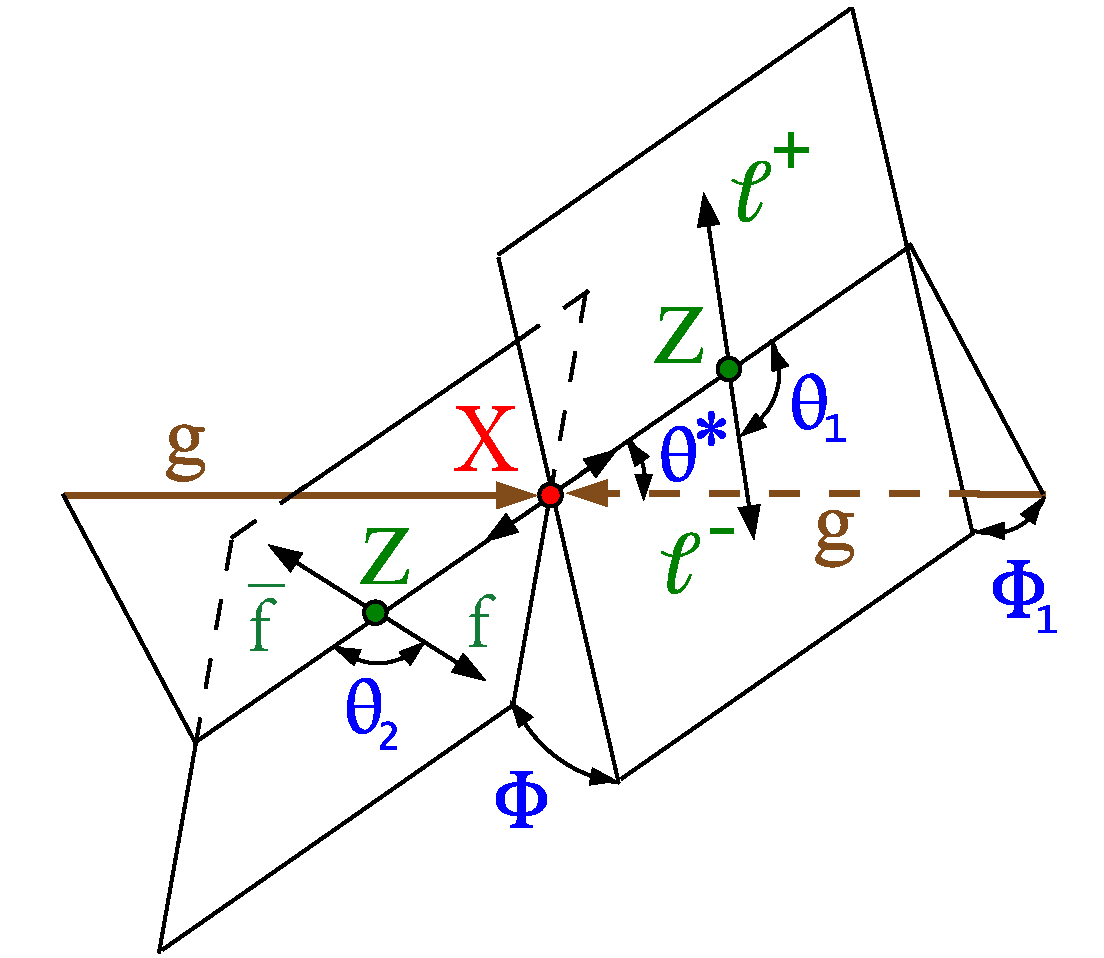
\includegraphics[width=0.45\textwidth]{figures/HighMassSearches/Figure_001-a.pdf}
    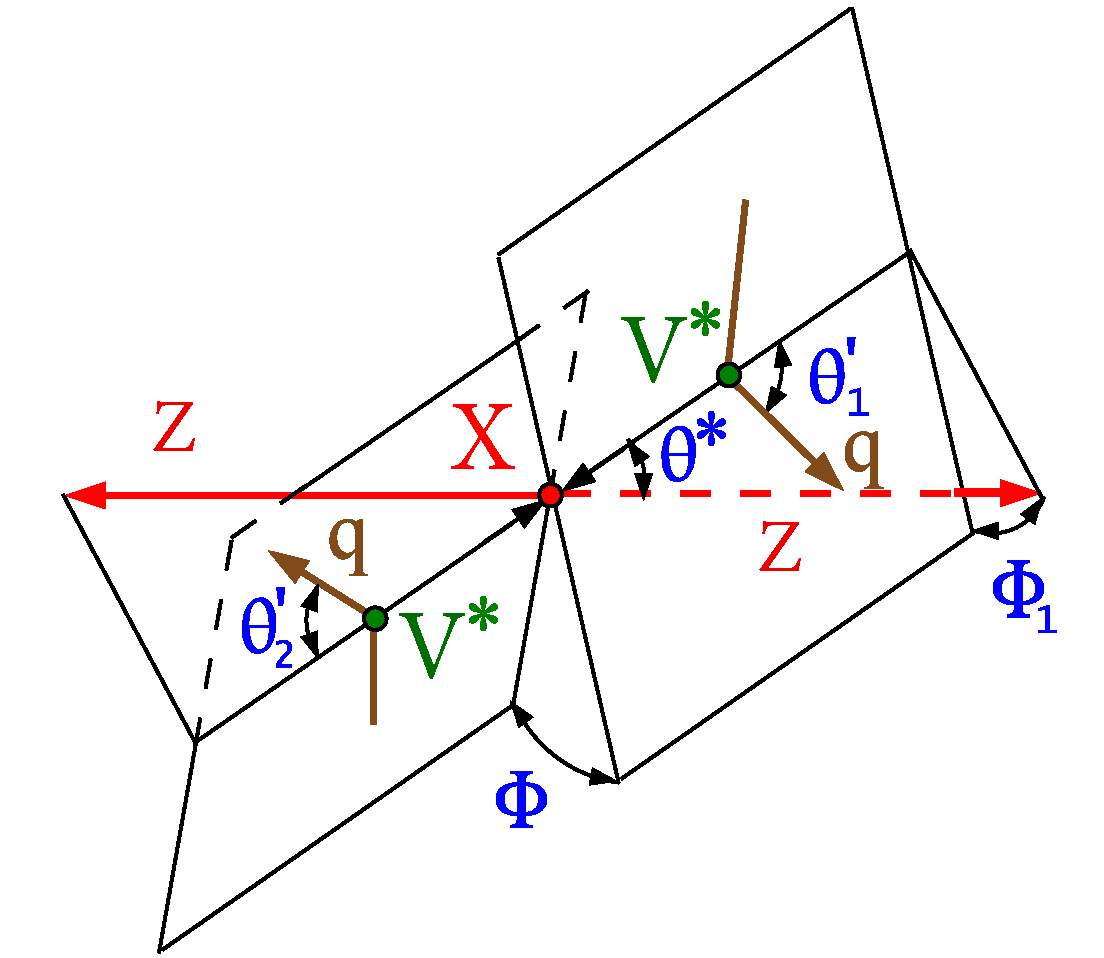
\includegraphics[width=0.45\textwidth]{figures/HighMassSearches/Figure_001-b.pdf}
    \caption
    {
    Illustration of an $\PX$ boson production from \ggF, $\Pg\Pg\to \PX\to \PZ\PZ\to (\ell^+\ell^-)(f\overline{f})$ (left), and VBF, $\Pq{\Pq^\prime}\to \Pq{\Pq^\prime} \PX \to \Pq{\Pq^\prime}\PZ\PZ$ (right). The five angles shown in blue and the invariant masses of the two vector bosons shown in green fully characterize either the production or the decay chain. The angles are defined in either the \PX\ or \PV\ boson rest frames~\cite{Gao:2010qx,Anderson:2013afp}.
    }
    \label{fig:decay}
\end{figure}

The discriminant sensitive to the $Z+JJ$ kinematics is calculated as
%%%%%%%%%%%%%%%%%%%%%
\begin{eqnarray}
\label{eq:Zjjmela}
\mathcal{D}_{\rm Zjj} =
\left[1+  \frac{  c_{\rm Zjj}\times{\cal P}_\text{Zjj} (\vec\Omega^{\PX\to2\ell2q} | m_{2\ell2q})}
{{\cal P}_{\PX\to2\ell2q} (\vec\Omega^{\PX\to2\ell2q} | m_{2\ell2q})} \right]^{-1}\,
\end{eqnarray}
%%%%%%%%%%%%%%%%%%%%%
where the denominator contains the probability of the signal
and the numerator includes the probability for the dominant $\PZ +jj$ background process,
all calculated either with the
$\JHUGEN{}$ (signal) or $\MCFM{}$ (background) matrix elements within the MELA framework.
The value of $c_{\rm Zjj}$ is tuned as a function of \mZZ{} in order to preserve good
the population of events in the range [0,1]. The template ${\cal T}(\mathcal{D}_{\rm Zjj}|m_{2\ell2q})$ used in the analysis is conditionally
normalised such that each slice of $\mathcal{D}_{\rm Zjj}$ is normalised to the unit area
for a given value of $m_{2\ell2q}$.

The discriminant sensitive to the VBF signal topology with two associated jets
is calculated as~\cite{Khachatryan:2015cwa, Khachatryan:2015mma}
%%%%%%%%%%%%%%%%%%%%%
\begin{eqnarray}
%
\label{eq:vbfmela}
\mathcal{D}_{2\rm jet} =
\left[1+
\frac{ c_{\rm XJJ}\times\mathcal{P}_{\rm XJJ} (\vec\Omega^{\rm \PX+JJ} | m_{2\ell2q}) }
{\mathcal{P}_{\rm VBF}  (\vec\Omega^{\rm \PX+JJ} | m_{2\ell2q})  }\right]^{-1}
\,,
%
\end{eqnarray}
%%%%%%%%%%%%%%%%%%%%%
where $\mathcal{P}_{\rm VBF}$ and $\mathcal{P}_{\rm \PX JJ}$ are probabilities obtained from the
\JHUGEN{} matrix elements for the VBF process and gluon fusion (technically a combination of
$gg/qg/qq^\prime$ parton collisions)
in association with two jets ($\PX+2$\,jets) within the MELA framework.
The value of $c_{\rm XJJj}$ is tuned as a function of mass to preserve good
the population of events in the range [0,1]. This discriminant help us in discriminating the VBF/ggH topology.

\section{Event reconstruction and selection}
\label{sec:EventSelection}
% This is my fig.~\ref{fig:test}.
% \begin{figure}[!htb]
%     \centering
%     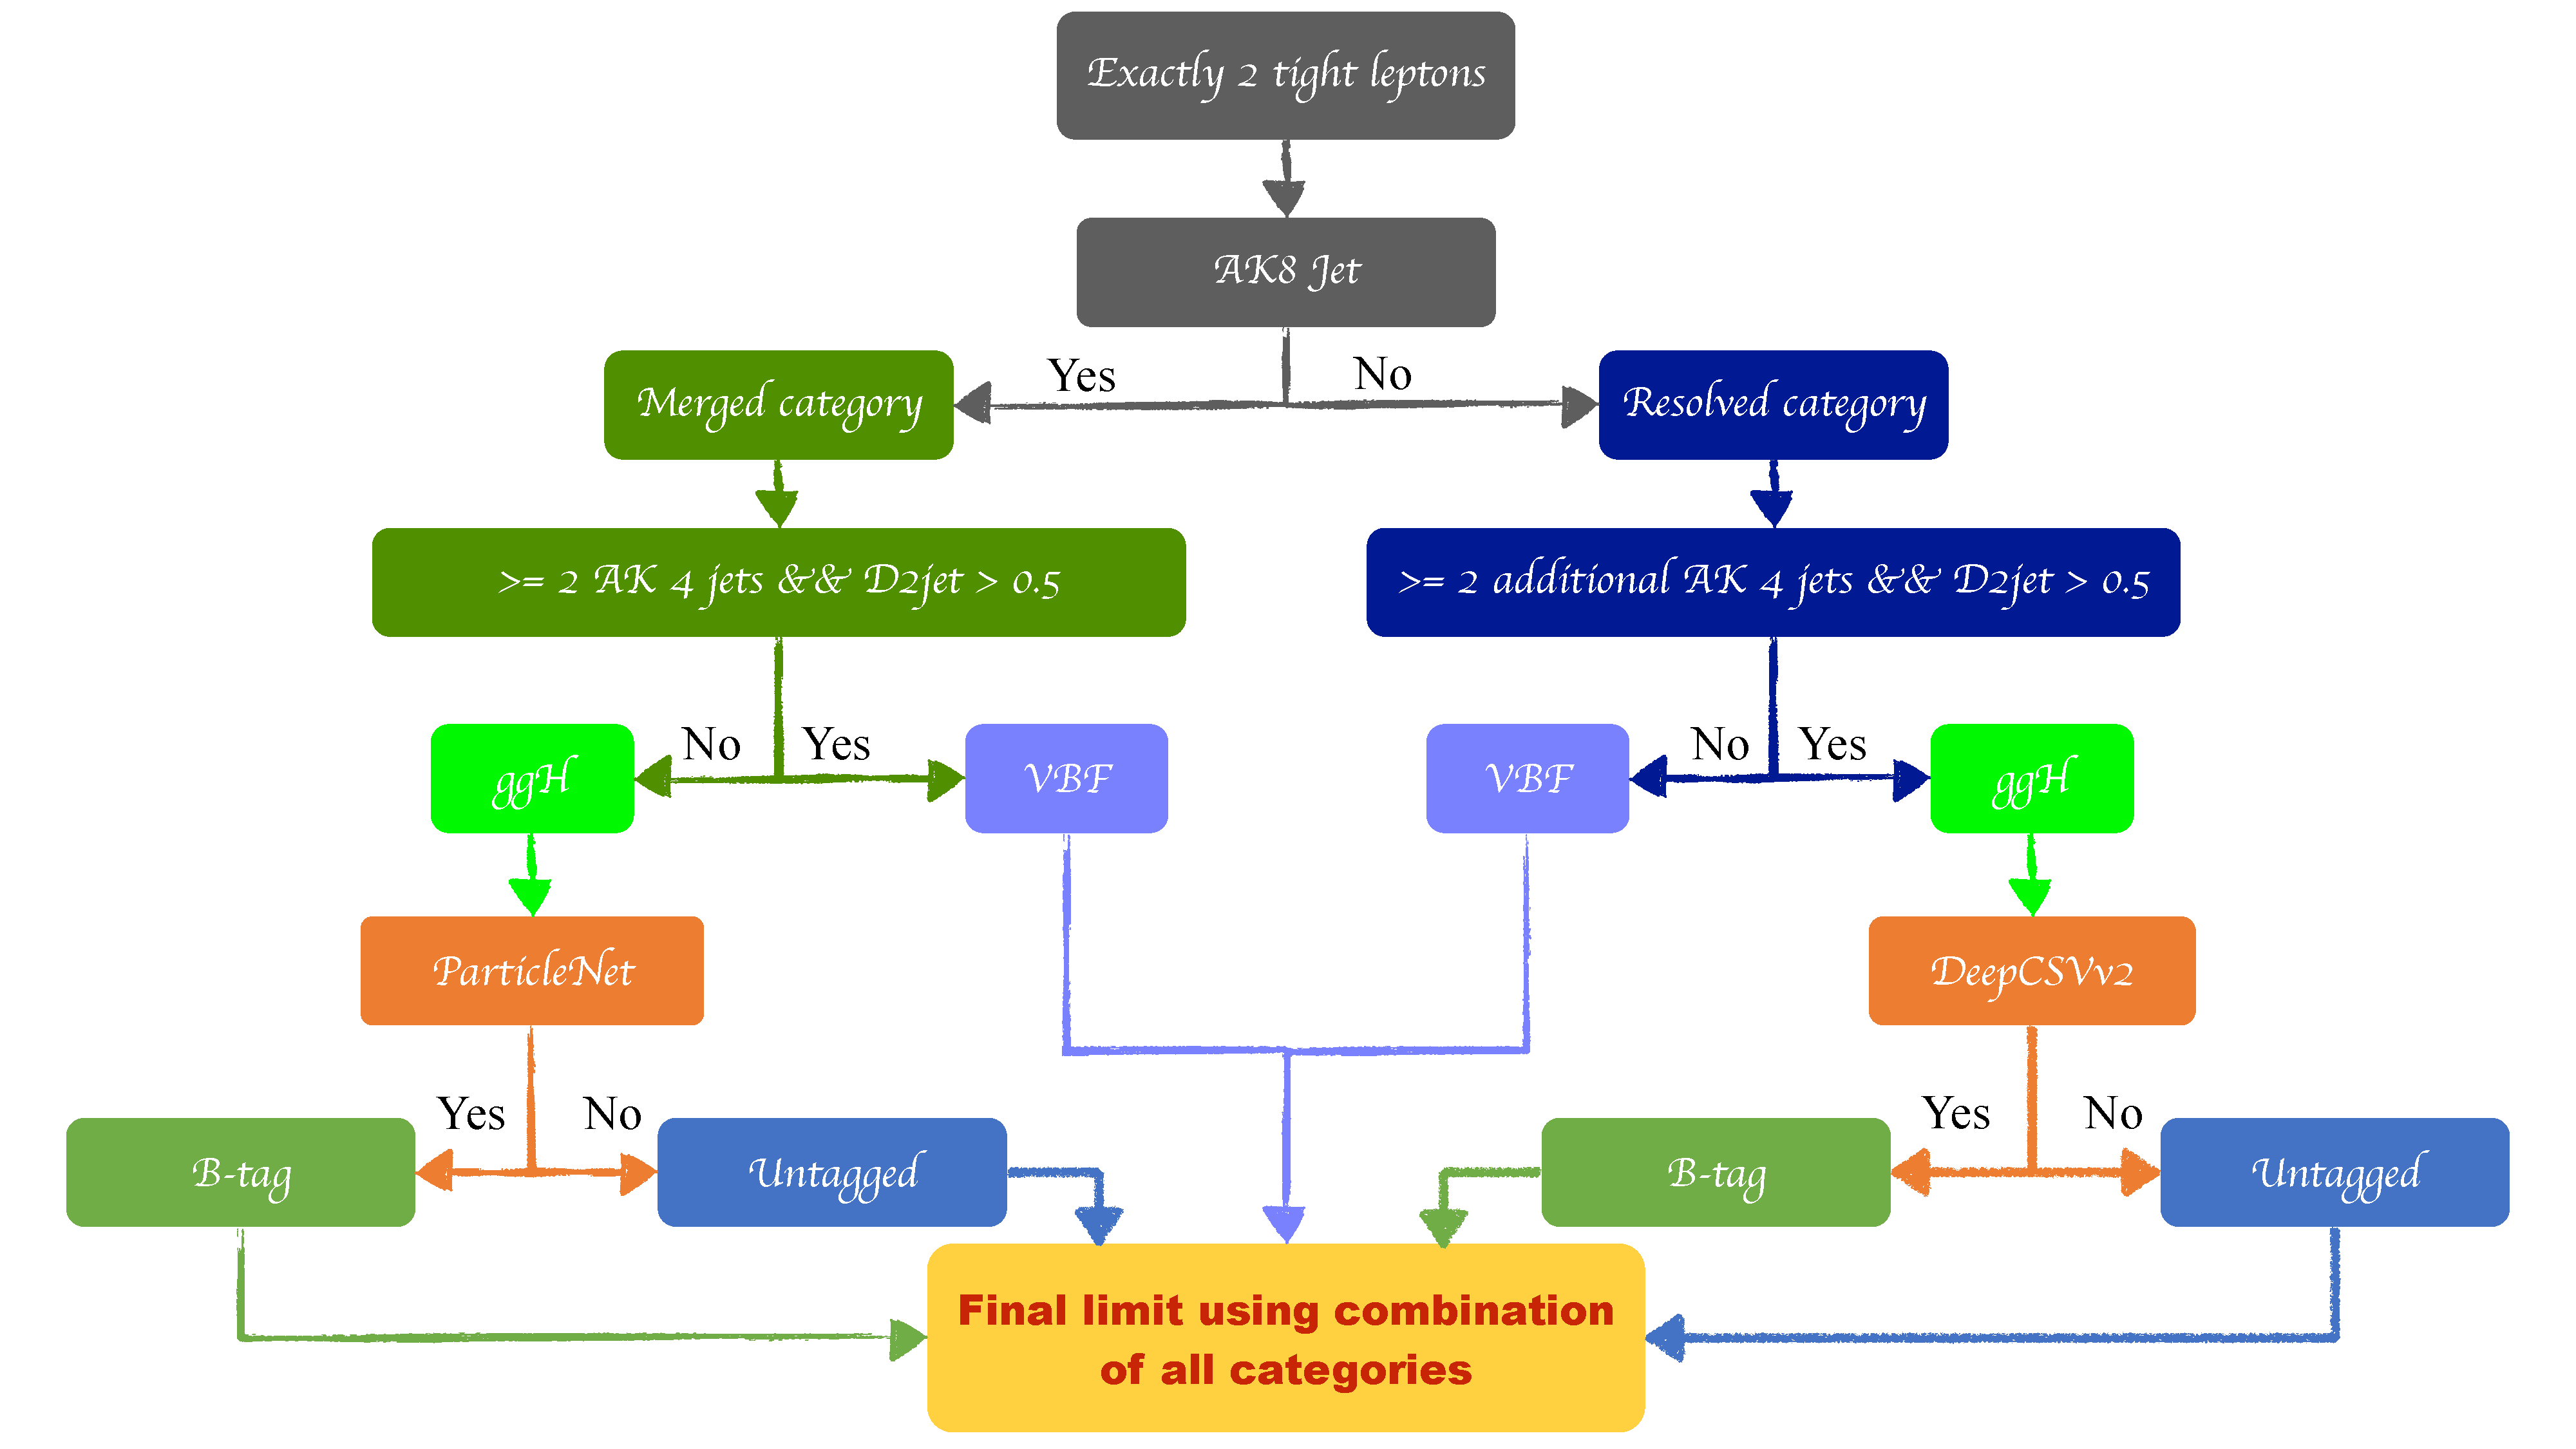
\includegraphics[width=\textwidth]{figures/HighMassSearches/ZZ2l2Q_FlowChart.pdf}
%     \caption[Caption for TOC]{Even selection flow chart.}
%     \label{fig:test}
% \end{figure}
%
In the CMS detector, the Particle-Flow (PF) algorithm~\cite{Sirunyan:2017ulk} is employed to reconstruct and identify individual particles as charged and neutral hadrons, leptons, and photons by combining information from all sub-detectors.
The primary vertex (PV) is defined as the vertex with the highest sum of squared transverse momenta from charged tracks.

The leptons considered are required to be associated with the PV of the event~\cite{Chatrchyan:2014fea} to suppress electron candidates originating from photon conversions and lepton candidates from in-flight decays of heavy quarks.
Additionally, leptons must be isolated from other particles in the event.
This analysis selects tight electrons or muons, defined as PF electrons or muons that pass a tight identification requirement, with an average efficiency of approximately 90%\todo{Check this number}.

An algorithm is used to recover the final state radiation (FSR) from leptons.
Photons reconstructed by the PF algorithm are considered as FSR candidates if they satisfy specific criteria, $\PT^{\Pgg} > 2\GeV$ and ${\cal I}^{\ell}< 1.8$~\cite{Sirunyan:2017exp}, and those that do not satisfy additional requirements are discarded.
The lowest candidate for every lepton is retained, and the photons identified as FSR are excluded from any isolation computations.

In addition to ID requirements, leading and sub-leading lepton candidates must have transverse momenta greater than 40 and 24 GeV, respectively, and a pseudorapidity in the range (0 $<$ $|\eta|$ $<$ 2.4), to remain in the CMS tracker region.

Jets are constructed using the anti-kT clustering method and are required to pass a loose identification criteria to reject jets from pileup interactions~\cite{antikt,Cacciari:2011ma}.
The considered jets should satisfy certain conditions and be separated from all selected leptons by a $\Delta R(\ell,\text{jet})>0.4$.
The analysis uses b-tagged jets, having $\abs{\eta^{\text{jet}}}<2.4$, for event categorization and selection, where a b-jet is tagged using the deep combined secondary vertex algorithm based on the impact parameter significance of the tracks associated with the jet~\cite{Chatrchyan:2012jua,CMS-PAS-BTV-15-001}. The loose working point is used, corresponding to an efficiency of 80\% and a mistag rate of 10\% for light quark jets.

The main feature distinguishing the two dominant $\PX$ boson production mechanisms (\ggF and VBF) is the presence of associated jets and the kinematic correlation between such jets and the $\PX$ boson.
Events are split into categories based on kinematic correlations to gain sensitivity to the production process of the $\PX$ boson.
A ME technique is employed to categorize events based on the correlation between the two forward jets and the $\PX$ boson candidate.
In this analysis, events are selected by combining leptonically and hadronically decaying \cPZ\ candidates.

The $\cPZ$ candidates are formed from pairs of leptons of the same flavor and opposite charge ($\Pe^{+}\Pe^{-}$, $\Pgm^{+}\Pgm^{-}$) and are required to pass the invariant mass selection $60 < m_{\ell^+\ell^-} < 120\GeV$.
A minimum dilepton transverse momentum, \PT{} of \unit{\DILEPTONPTCUT}{\GeV}, is imposed to reject Drell-Yan events with small hadronic recoil.

Hadronically decaying $\cPZ$ boson candidates (\Zhad) are reconstructed using two distinct techniques, referred to as "resolved" and "merged."
In the resolved case, the two quarks from the $\cPZ$ boson decay form two distinguishable AK4 jets, while in the merged case, a single AK8 jet with a large transverse momentum is taken as a \Zhad.

In the merged jet case, a pruning algorithm is applied to the AK8 jet to recluster the jet constituents while applying additional requirements that eliminate soft, large-angle QCD radiation that artificially increases the jet mass relative to the nominal $\cPZ$ boson mass~\cite{prune,substructure}.

Jets must not overlap with leptons, so a cut on $\Delta R(\ell, jet) > 0.4~(0.8\textrm{~for merged})$ is applied to resolved and merged jets.
Finally, the reconstructed events are required to have an invariant mass around the $\cPZ$ boson mass: $\LSBLOW < \MZhad < \unit{\USBHIGH}{\GeV}$.
Among this, the region 70--105 GeV is considered the signal region, while the regions 40--70 GeV and 135--180 GeV form the sideband region.
The region with possible $\Ho \to \bbbar$ signals, 105--135 GeV, is removed from any selection.
Furthermore, a $\PT > \unit{\VHADRESOLVEDPTCUT}\ (\VHADMERGEDPTCUT) {\GeV}$ is applied in the resolved (merged) case.
Finally, we consider events with $m(\ell\ell J) > 100$ GeV.%\todo{Check the mZZ cut}

To minimise contamination from standard model DY + jets production and QCD, we further require that the hadronic Z boson candidate from a merged selection has a substructure.
The ParticleNet tagger is exploited to ensure that the candidate has substructure.

The selection preference is given to merged jets when multiple categories are present. If no merged jets are found, the resolved category is considered.
Within each selection category, the candidate with the largest transverse momentum has priority over the others.

The hadronically and leptonically decaying $\cPZ$ boson candidates are combined to form a resonance candidate.
The reconstructed $\cPZ\cPZ$ candidate mass (\mZZ{}) denotes the dilepton + dijet mass (\mlljj{}) in the resolved case and the dilepton + merged jet invariant mass (\mllJ{}) in the merged case.
A requirement of $\mZZ{}> \unit{\MZZCUT}{\GeV}$ is imposed to reduce the $\cPZ + \text{jets}$ background.%\todo{Check}

To increase sensitivity to different production modes, events are categorized into VBF and inclusive types.
Furthermore, a dedicated category is defined for events enriched with \cPqb\ quark jets due to the presence of $\cPZ\to\bbbar$ decays. The definitions are as follows:
\begin{itemize}
	\item  \textbf{VBF-tagged} requires two additional and forward jets besides those constituting the hadronic $\cPZ$ boson candidate; a mass dependent selection criterion on ${\cal D}^\mathrm{VBF}_{\mathrm{2jet}}$ is applied;
	\item  \textbf{\cPqb\ tagged} consists of the remaining events with two \cPqb\ tagged jets (in the resolved case) or two \cPqb\ tagged subjets from the hadronic $\cPZ$ boson candidate;
	\item  \textbf{Untagged} consists of the remaining events.
\end{itemize}

As a result of this categorization, events are split into twelve categories: $2\Pe 2\Pq$ or $2\mu 2\Pq$, either VBF-tagged, b-tagged, or untagged, and each with either merged jets or resolved jets.
Each event is characterized by the two observables ($\mZZ$, $\ZJJMELA$). The invariant mass distribution for merged and resolved events in each category after the selection is shown in Fig~\ref{fig:ZZmass_untag}. The \ZJJMELA and \VBFMELA distributions for resolved events in each category together after the selection are shown in Fig.~\ref{fig:ZZmela_untag}.

\begin{figure}[htbp]
    \centering
    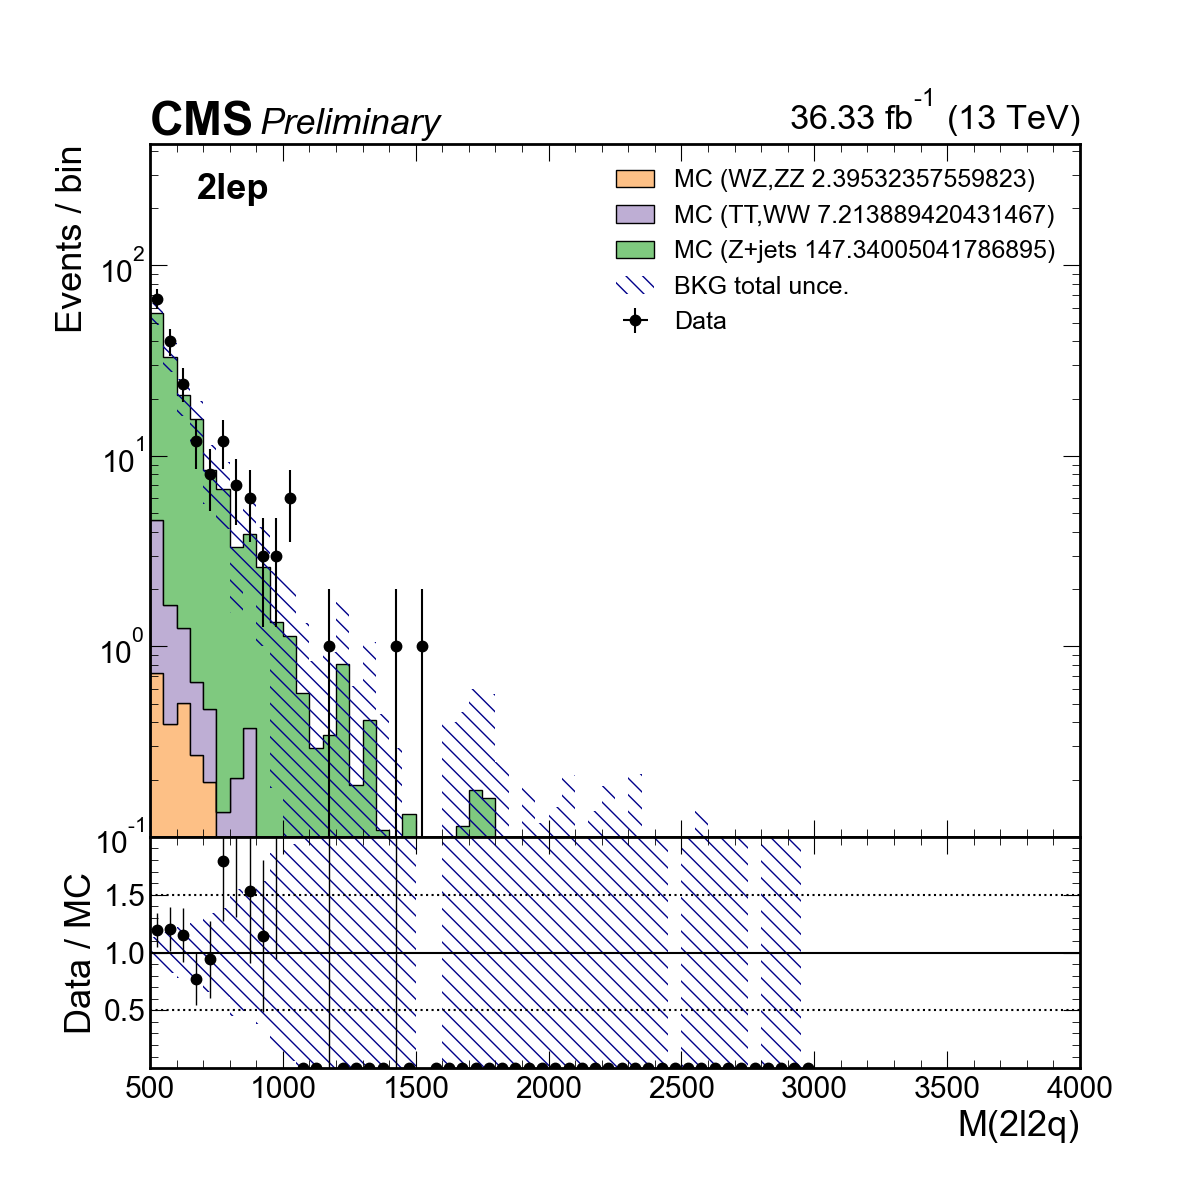
\includegraphics[width=0.45\textwidth]{figures/HighMassSearches/dataMCPlots/mass2l2jet_CR_2lep_btag.png}
    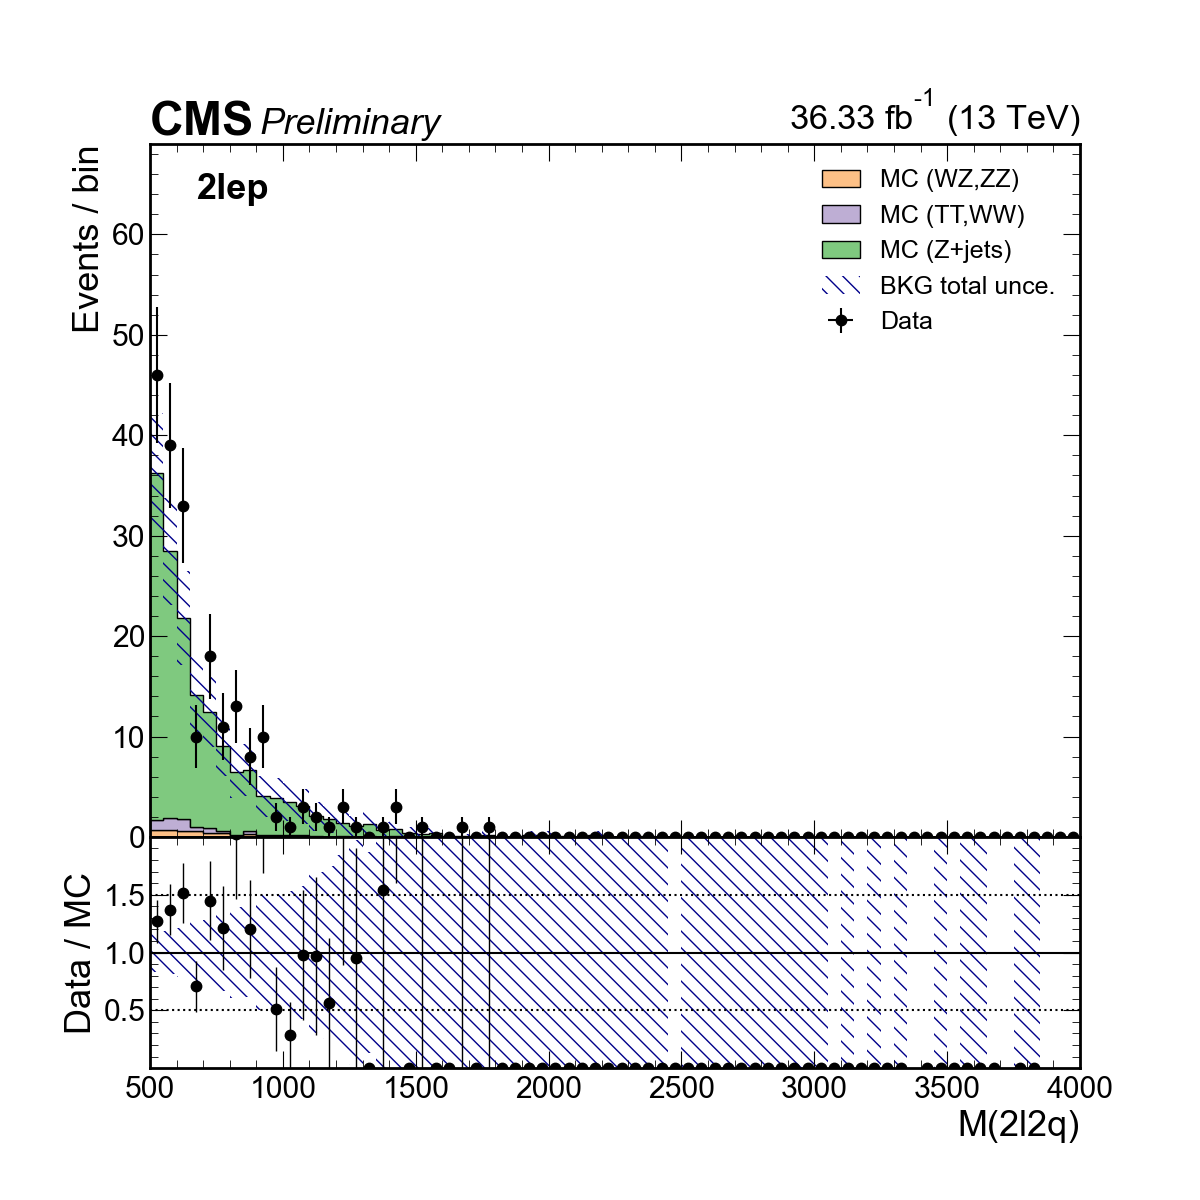
\includegraphics[width=0.45\textwidth]{figures/HighMassSearches/dataMCPlots/mass2lj_CR_2lep_btag.png}\\
    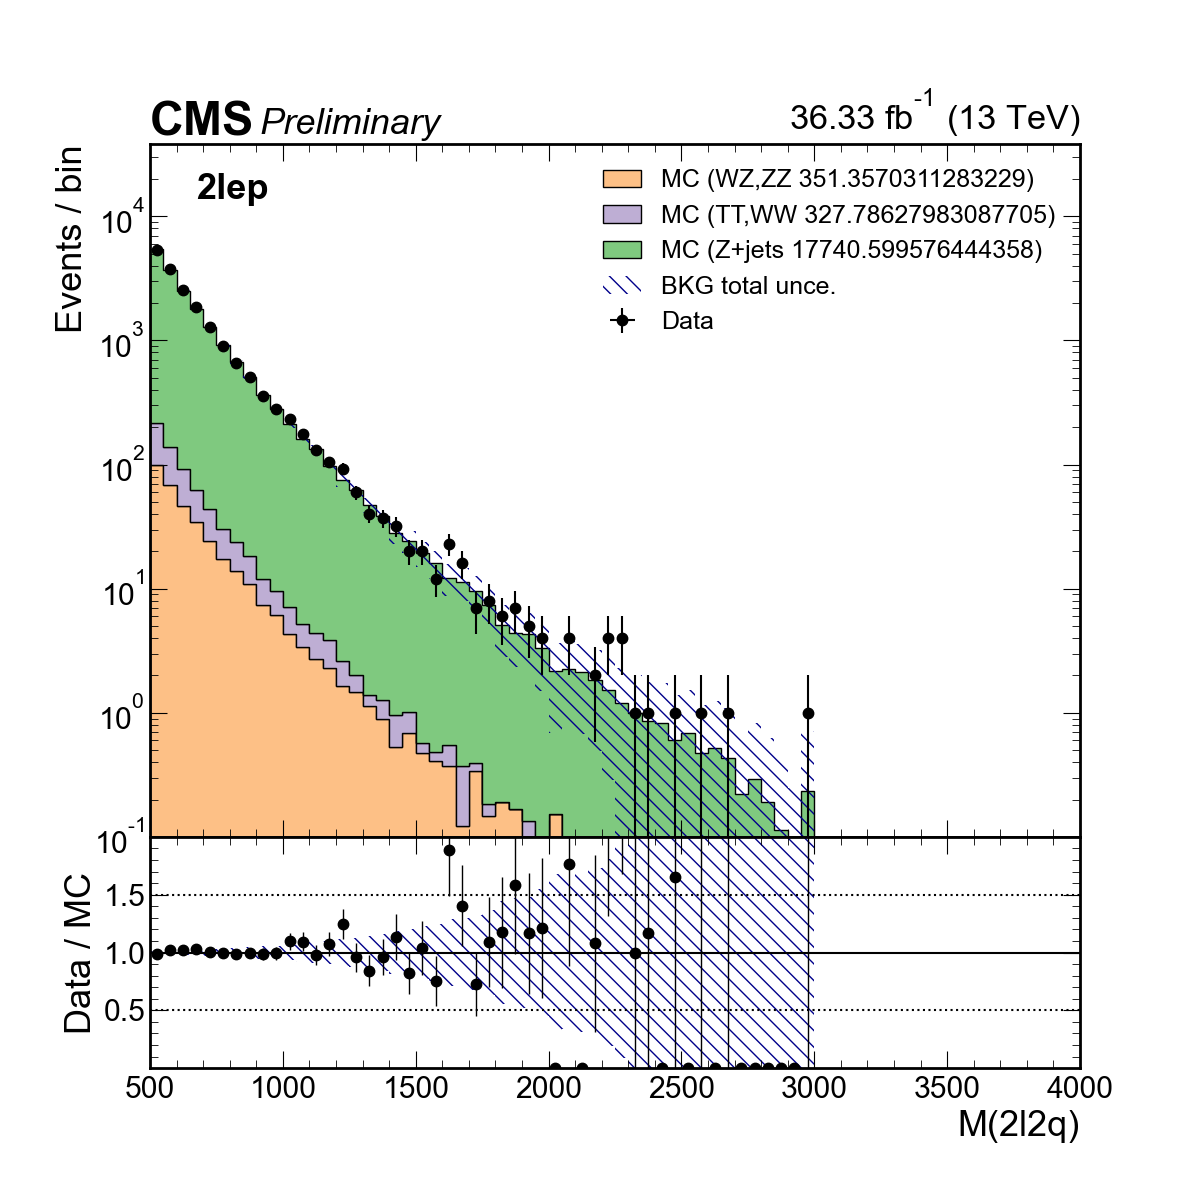
\includegraphics[width=0.45\textwidth]{figures/HighMassSearches/dataMCPlots/mass2l2jet_CR_2lep_untag.png}
    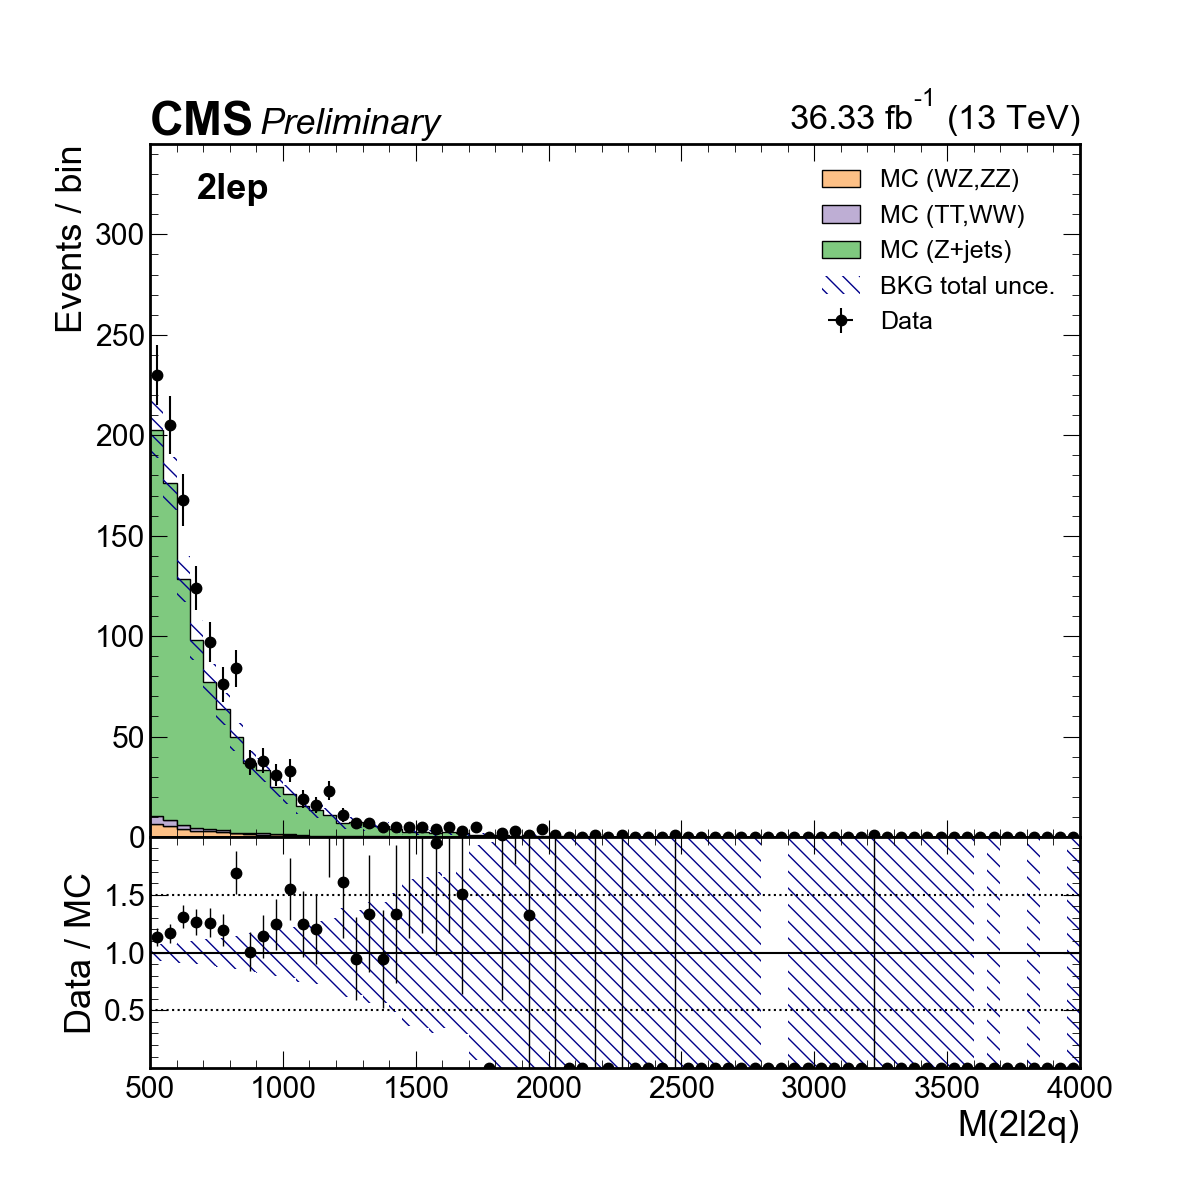
\includegraphics[width=0.45\textwidth]{figures/HighMassSearches/dataMCPlots/mass2lj_CR_2lep_untag.png}
    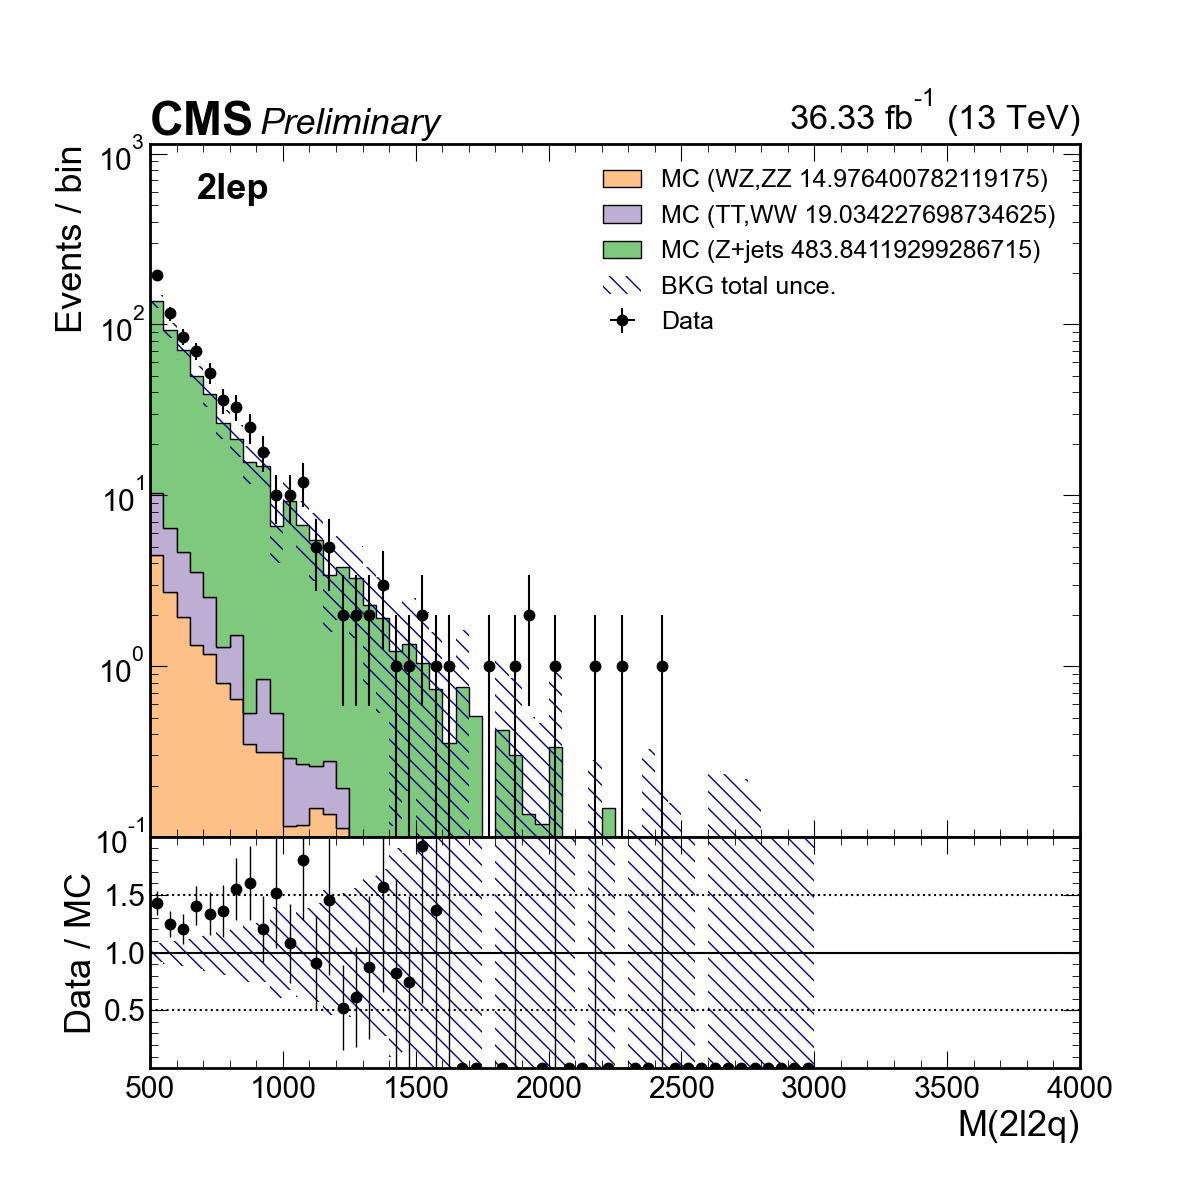
\includegraphics[width=0.45\textwidth]{figures/HighMassSearches/dataMCPlots/mass2l2jet_CR_2lep_vbftag.png}
    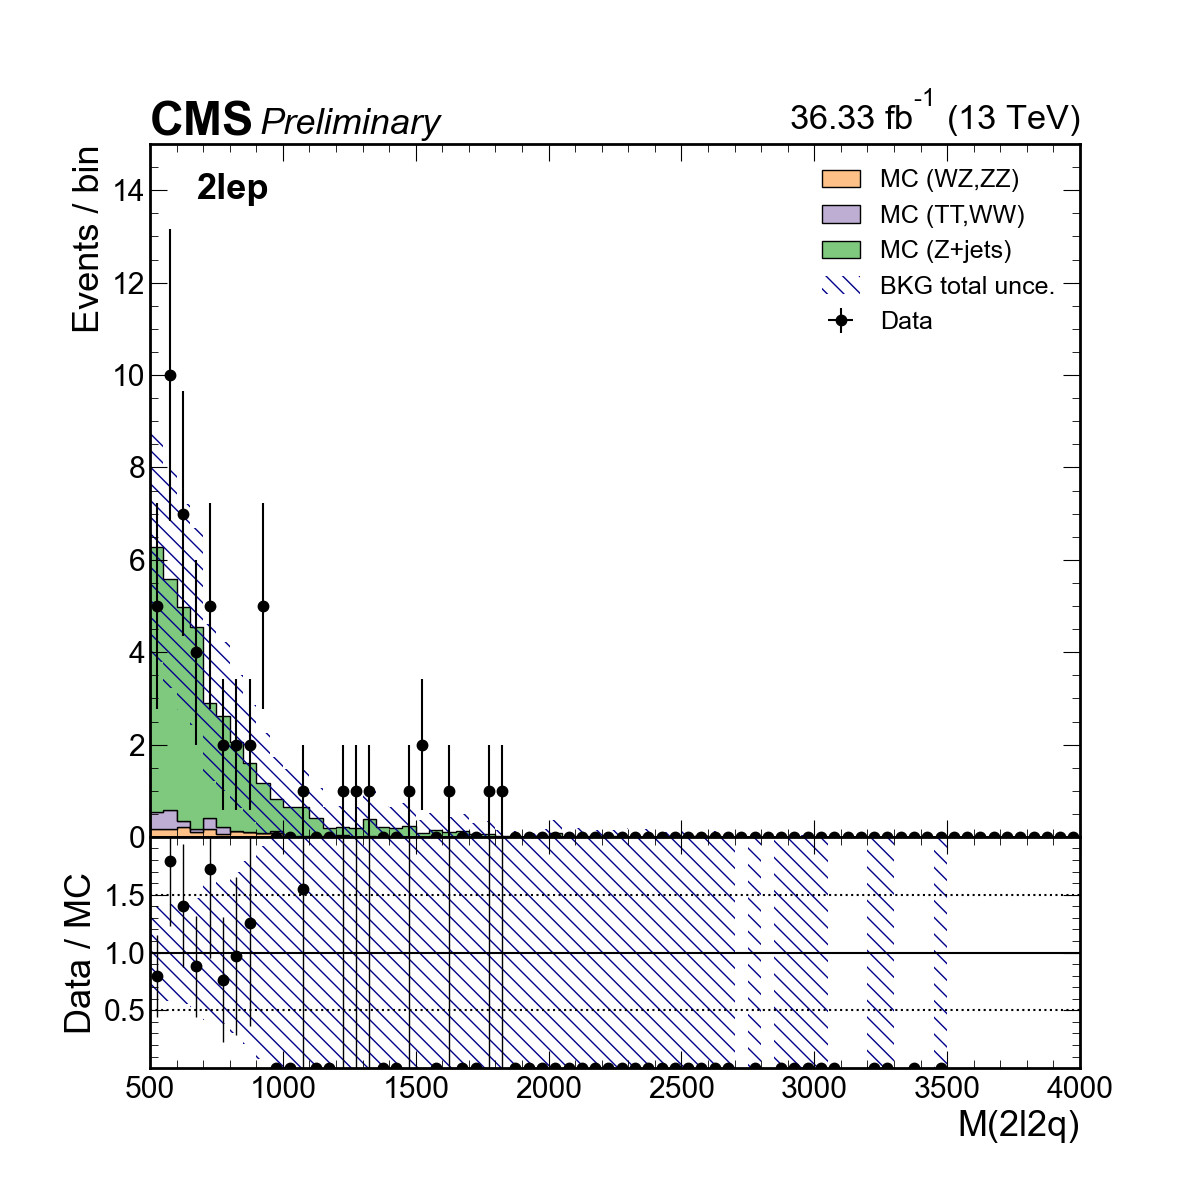
\includegraphics[width=0.45\textwidth]{figures/HighMassSearches/dataMCPlots/mass2lj_CR_2lep_vbftag.png}\\

    \caption{Distributions of the invariant mass \mZZ{} in the control region for the merged (right) and resolved (left) case for the different categories in the $2{\ell}2\Pq$ channel for 2016.
    % The points represent the data, the stacked histograms the expected backgrounds from simulation, and the open histograms the expected signal. The blue hatched bands refer to the sum of background estimates derived from either simulation or control samples in data, as described in the text.
    Lower panels show the ratio between data and background estimation in each case.
    }
    \label{fig:ZZmass_untag}
 \end{figure}

 \begin{figure}[htbp]
    \centering
    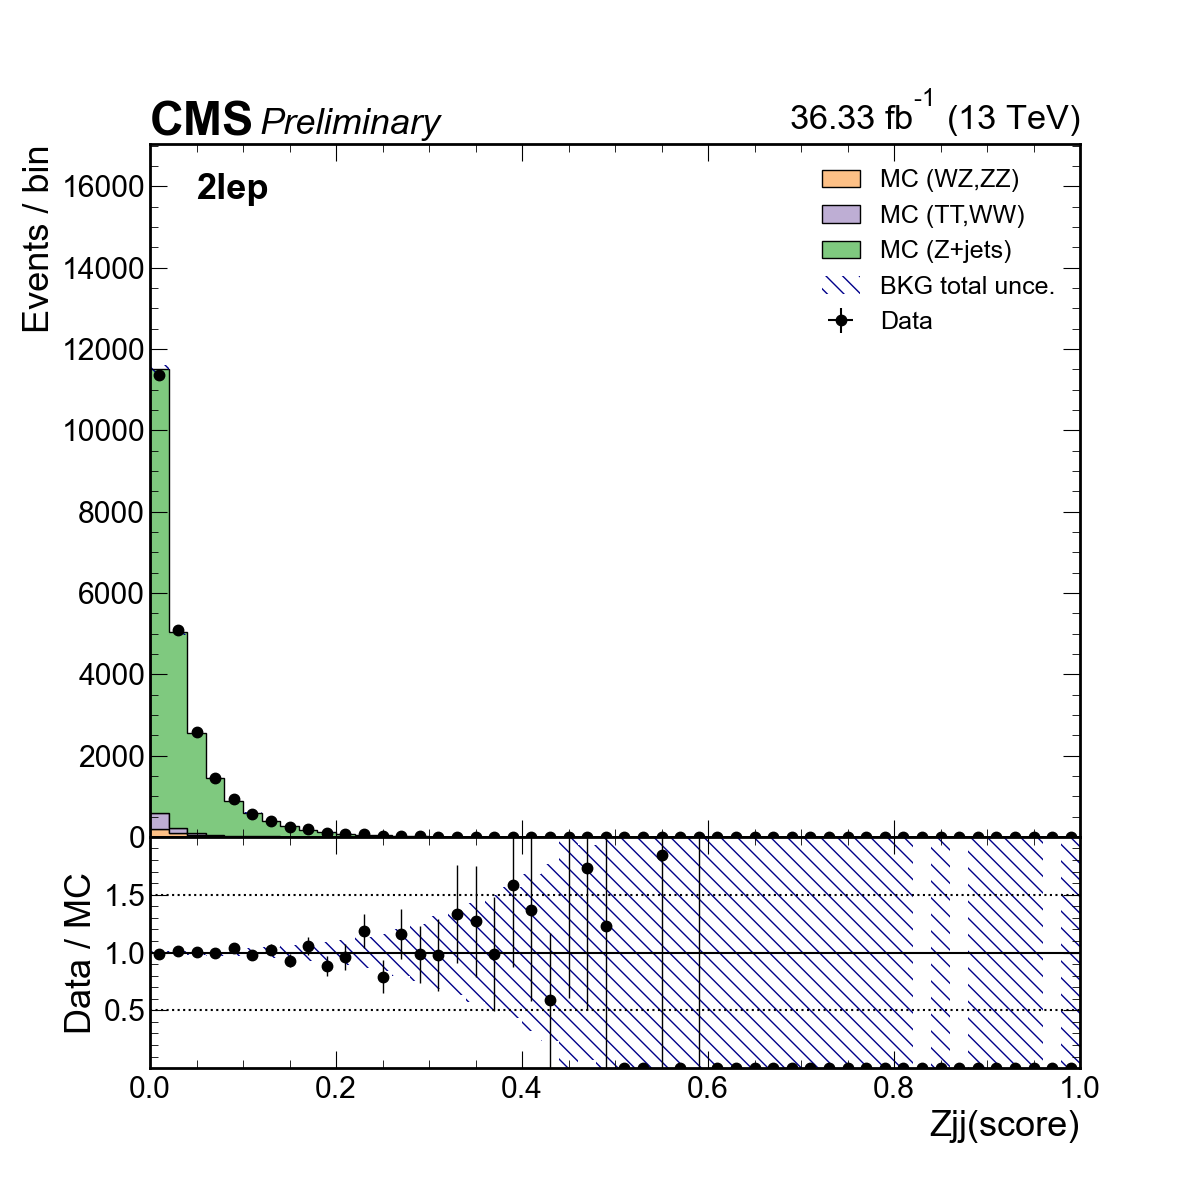
\includegraphics[width=0.45\textwidth]{figures/HighMassSearches/dataMCPlots/KD_ZJ_2lep.png}
    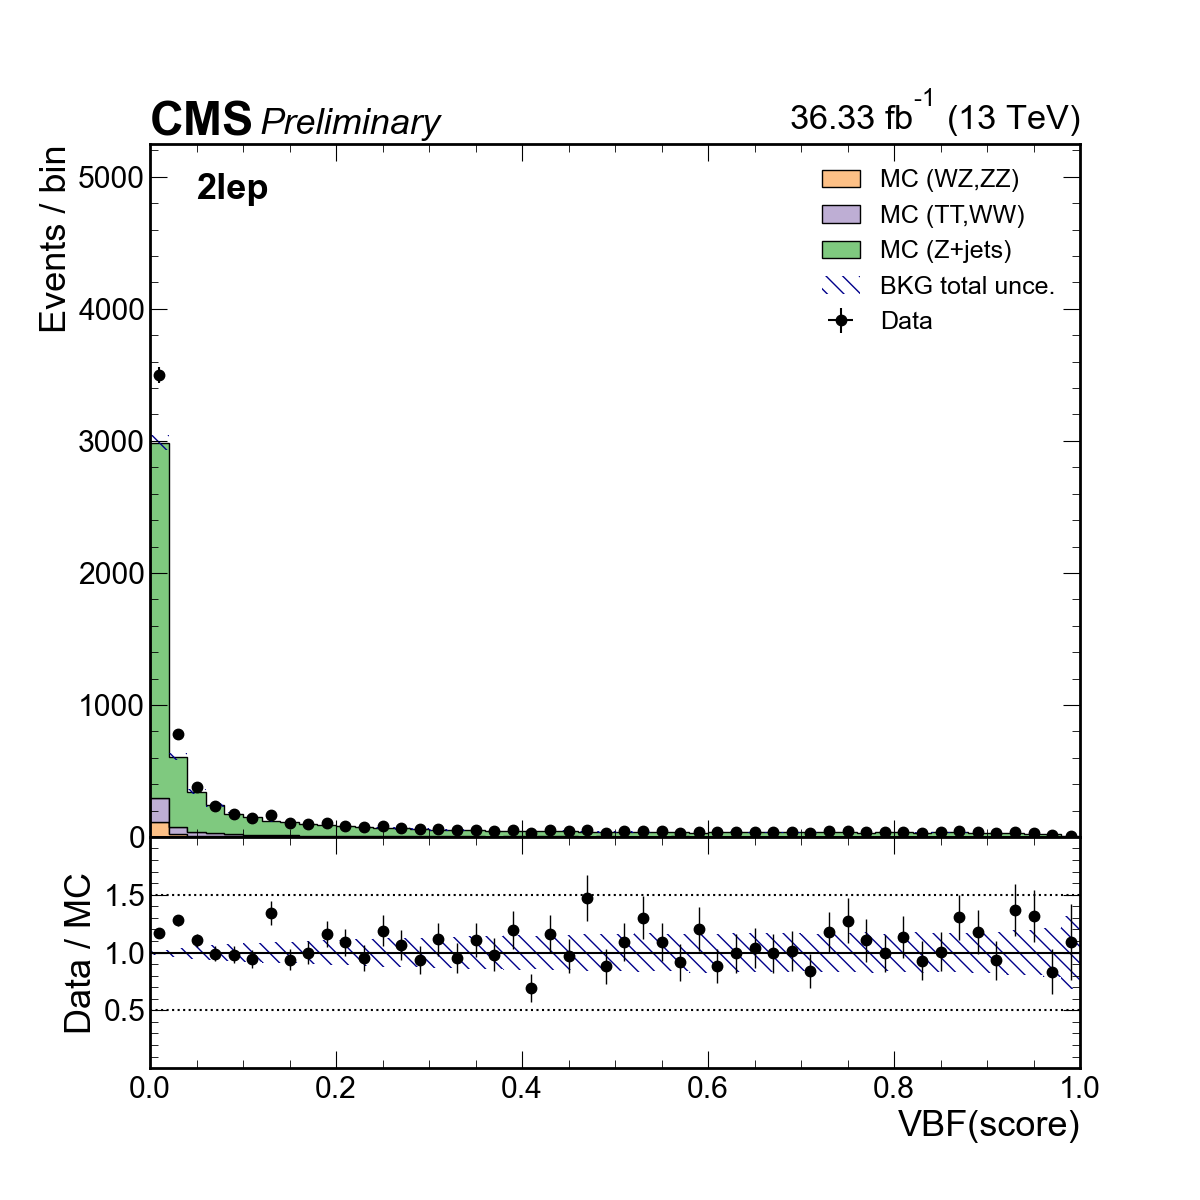
\includegraphics[width=0.45\textwidth]{figures/HighMassSearches/dataMCPlots/KD_JVBF_2lep.png}\\
    \caption{Distributions of the \ZJJMELA (left) and \VBFMELA (right) discriminants in the control region for the merged selection. The points represent the data, the stacked histograms the expected background from simulation.
    % , and the open histograms the expected signal.
    }
    \label{fig:ZZmela_untag}
 \end{figure}

 \section{Signal and background parameterization}
 \label{Section_parameterization}

 The goal of the analysis is to determine if a set of $\PX$ boson parameters
 $\mX$, $\GX$, and $\sigma_i\mathcal{B}_{X\to\cPZ\cPZ}$ is consistent with the data, where $\sigma_i\mathcal{B}_{X\to\cPZ\cPZ}$ is the product of the signal production cross section and
 the $\PX\to\cPZ\cPZ$ branching fraction in each production channel $i$ (gluon fusion or EW production). In practice, the $\sigma_i\mathcal{B}$ for $i=1,2$ are expressed in terms of
 $\sigma_{\mathrm{tot}}\mathcal{B}_{X\to\cPZ\cPZ}$ and $f_{\mathrm{VBF}}$, where $\sigma_{\mathrm{tot}}$ is the sum of the cross sections in the two production channels. The confidence intervals on $\sigma_{\mathrm{tot}}\mathcal{B}_{X\to\cPZ\cPZ}$
 are determined from profile likelihood scans for a given set of parameters $(\mX, \GX, f_{\mathrm{VBF}})$.
 The extended likelihood function is defined for candidate events as
 \begin{eqnarray}
 \mathcal{L} =  \exp\Big( - \sum_{i} n_{vv}^i -\sum_i n_\text{bkg}^i  \Big)
 \prod_k \prod_j
 \Big(
   \sum_i n_{vv}^{i} \mathcal{P}^{i,k}_{vv}(\vec{x}_{j}; \mX, \GX)
 +\sum_i n_\text{bkg}^{i} \mathcal{P}^{i,k}_\text{bkg}(\vec{x}_{j})
 \Big),
 \label{eq:likelihood}
 \end{eqnarray}
 where $n_{vv}^i$ and $n_\text{bkg}^i$ are the numbers of signal and background events in channel $i$. The observables $\vec{x}_j$ are defined for each event $j$ in category $k$.
 % as discussed in Sections~\ref{sec:XZZ4l}, \ref{sec:XZZ2l2q}, and~\ref{sec:XZZ2l2nu}.
 There are several signal and background types~$i$, defined for each production mechanism.
 The background processes that do not interfere with the signal are described by the probability density functions (pdfs)
  $\mathcal{P}^{i,k}_\text{bkg}(\vec{x}_{j})$. The $vv\to \ff$ process is described by the pdf
 $\mathcal{P}^{i,k}_{vv}(\vec{x}_{j}; \mX, \GX)$ for $vv=\Pg\Pg$ (gluon fusion) and $vv= $ VV (EW production).
 This pdf describes the production and decay of the $\PX$ boson signal, SM background, including $\PH(125)$, and interference between all these contributions
 and is parameterized as follows:
 \begin{eqnarray}
 \mathcal{P}^{i,k}_{vv} (\vec{x}_{j}; \mX, \GX) =
 \mu_i  \mathcal{P}^{i,k}_{vv\to \PX\to \ff} (\vec{x}_{j}; \mX, \GX)
 + \sqrt{\mu_i}  \mathcal{P}^{i,k}_{\mathrm{int}} (\vec{x}_{j}; \mX, \GX)
 + \mathcal{P}^{i,k}_{vv\to\ff} (\vec{x}_{j})
 ,
 \label{eq:psig}
 \end{eqnarray}
 where $\mu_i$ is the relative signal strength for production type $i$ defined as the ratio of
 $\sigma_i\mathcal{B}$ with respect to a reference value, for which normalization of the pdf is determined.
 The interference contribution $\mathcal{P}^{i,k}_{\mathrm{int}}$ scales as $\sqrt{\smash[b]{\mu_i}}$ and the pure signal as ${\mu_i}$,
 while both depend on the signal parameters $\mX$ and $\GX$.
 The likelihood defined in Eq.~(\ref{eq:likelihood}) is maximized with respect to the nuisance parameters,
 which include the constrained parameters describing the systematic uncertainties.

 \subsection{Signal model}
 \label{sec:Signalmodel}

 The parameterization of $\mathcal{P}^{i,k}_{vv} (\vec{x}_{j}; \mX, \GX)$ is performed using the MC simulation
 discussed in Section~\ref{sec:MC} with the ME method.

 We parameterize the signal mass shape as follows:
 A pdf after detector effects ${\cal M}^{\mathrm{reco}}_{vv}(m_{\cPZ\cPZ})$ is implemented with the multiplicative efficiency function  ${\cal E}(m_{\cPZ\cPZ})$ and convolved with a mass resolution function
 ${\cal R}(m_{\cPZ\cPZ}|m^{\mathrm{Gen}}_{\cPZ\cPZ})$, both extracted from simulation of the \ggF and VBF processes:

 \begin{eqnarray}
 {\cal M}^{\mathrm{reco}}_{vv}(m_{\cPZ\cPZ})=
 \left({\cal E}(m_{\cPZ\cPZ}^{\mathrm{Gen}}) {\cal M}_{vv}(m^{\mathrm{Gen}}_{\cPZ\cPZ}|\mX,\GX)\right) \otimes {\cal R}(m_{\cPZ\cPZ}|m^{\mathrm{Gen}}_{\cPZ\cPZ}).
 \label{eq:signalpdf1D}
 \end{eqnarray}

 The parameterizations of ${\cal R}(m_{\cPZ\cPZ}|m^{\mathrm{Gen}}_{\cPZ\cPZ})$ and ${\cal E}(m_{\cPZ\cPZ}^{\mathrm{Gen}})$ cover the mass
 range from 500\GeV to 3\TeV. Figure~\ref{fig:eff} shows the efficiencies in the various categories. The resolution is 3--5\%. With the above ingredients, the $m_{\cPZ\cPZ}$ parameterization is shown in Fig.~\ref{fig:mzz_interference}, for a boson with $\mX = 500\GeV$, $\GX = 15\GeV$.
 % The interference contributions from $\PH(125)$ and $\Pg\Pg\to\cPZ\cPZ$ background are also shown.

 \begin{figure}[htbp]
 \centering
 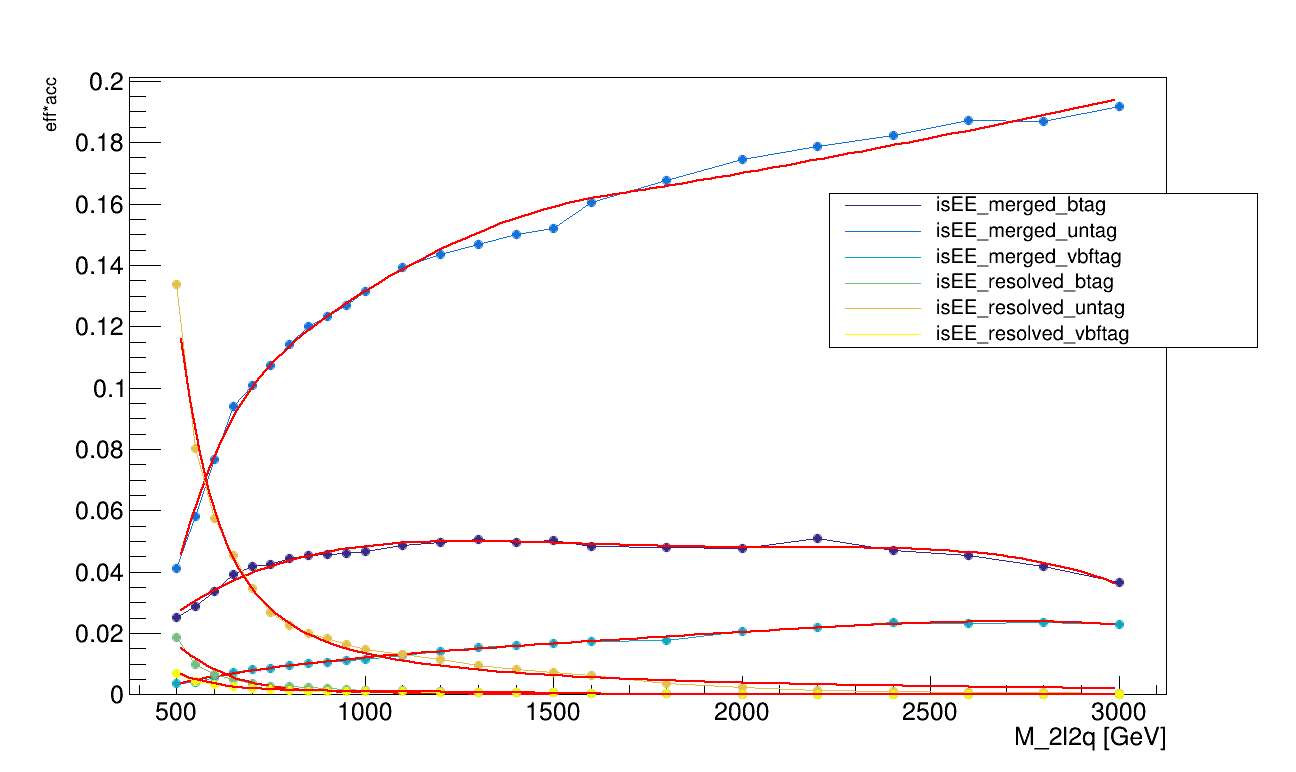
\includegraphics[width=0.45\textwidth]{figures/HighMassSearches/Efficiency/eff_ggh_isEE.png}
 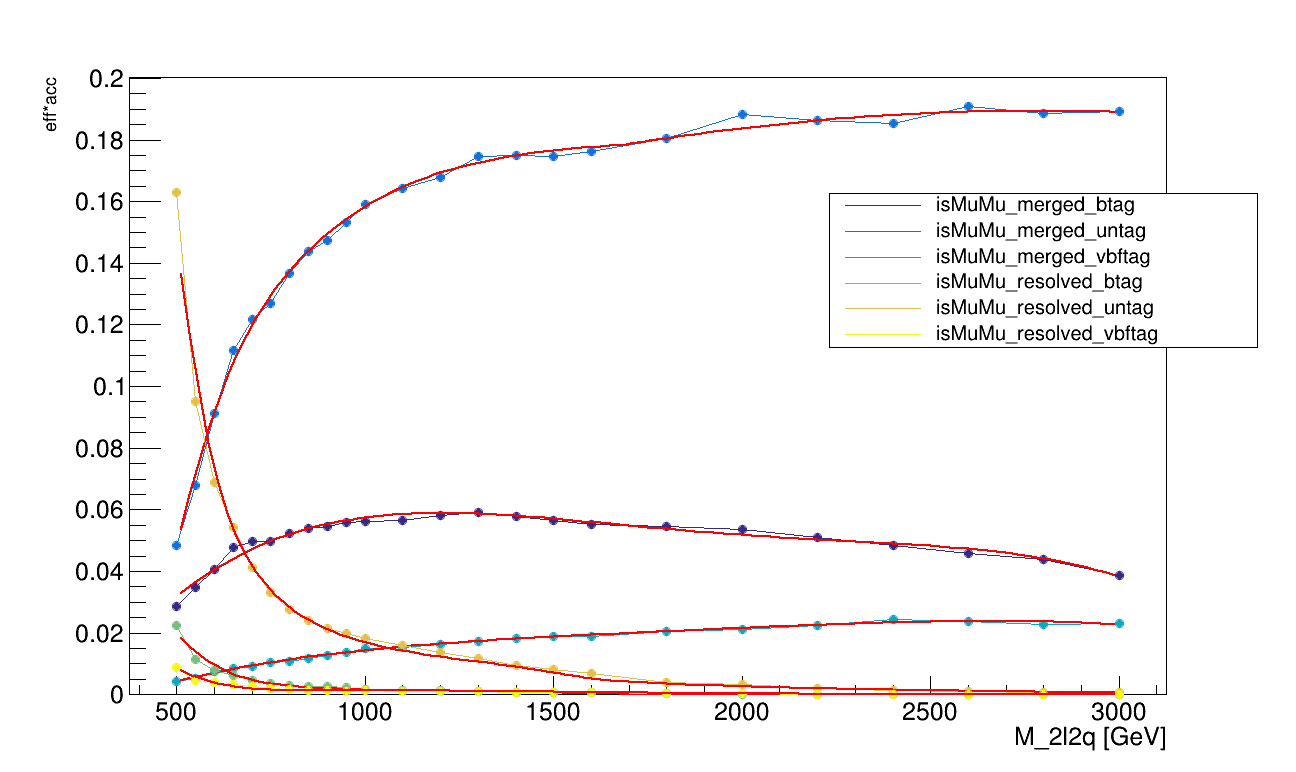
\includegraphics[width=0.45\textwidth]{figures/HighMassSearches/Efficiency/eff_ggh_isMuMu.png}\\
 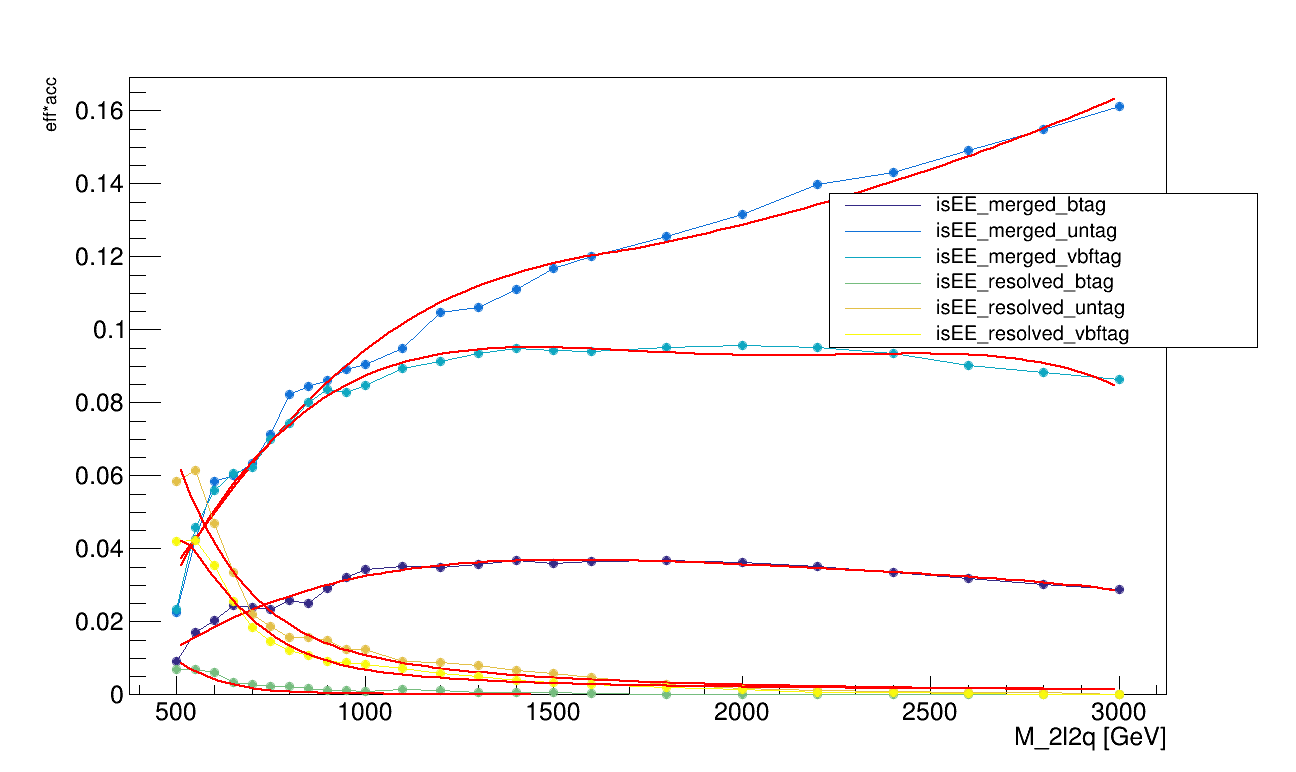
\includegraphics[width=0.45\textwidth]{figures/HighMassSearches/Efficiency/eff_vbf_isEE.png}
 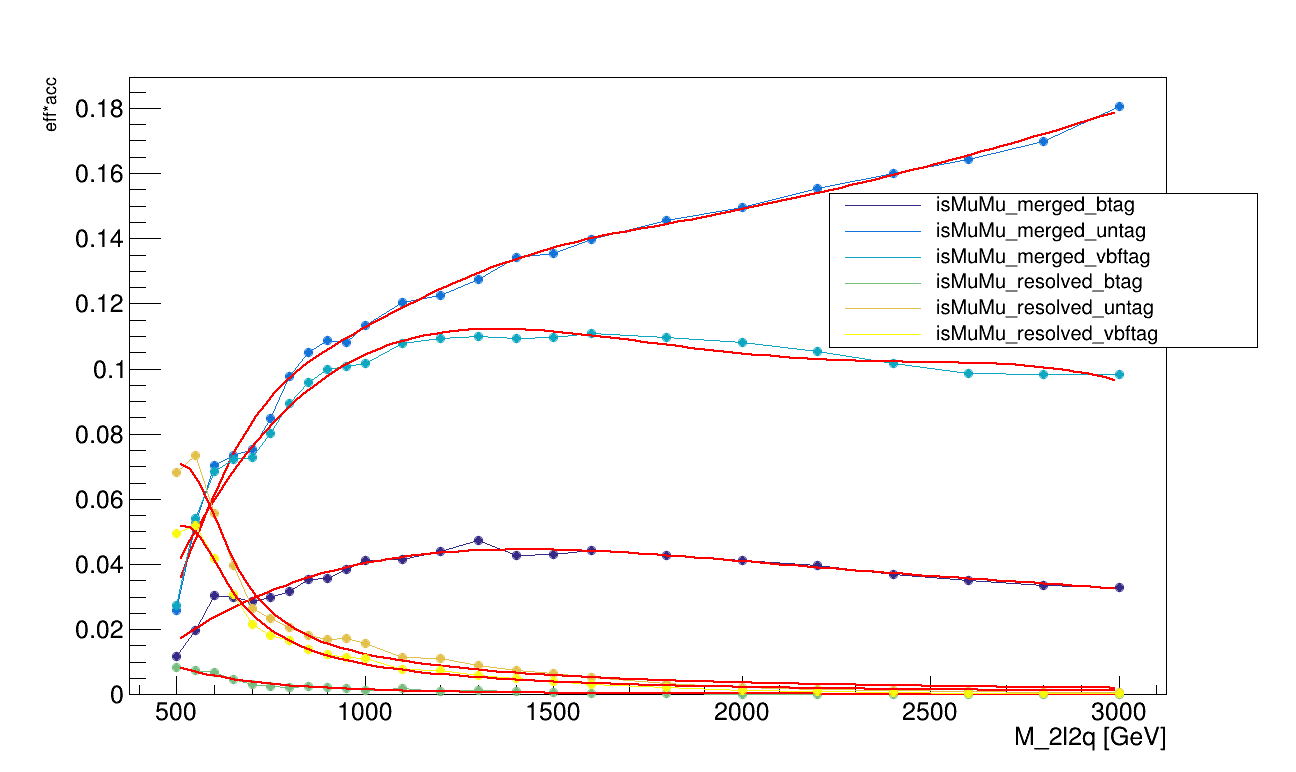
\includegraphics[width=0.45\textwidth]{figures/HighMassSearches/Efficiency/eff_vbf_isMuMu.png}\\
     % \missingfigure{efficiency plot}
 \caption{
     The product of efficiency and acceptance for signal events to pass selection as a function of the generated mass $m_{\cPZ\cPZ}^{\mathrm{Gen}}$, for \ggF (top) and VBF (bottom) production modes.
     The left panels represent the electron channels, while the right panels correspond to the muon channels.
 \label{fig:eff}
 }
 \end{figure}

 The 2D signal distributions in the final states are built with the conditional template ${\cal T}(\Dbkg|m_{\cPZ\cPZ})$,
 which describes the $\Dbkg$ discriminant distribution from Eq.~(\ref{eq:Dbkgmela}) or~(\ref{eq:Zjjmela})
 for each value of $m_{\cPZ\cPZ}$:

 \begin{eqnarray}
 {\cal P}^{i, k}_{vv}(m_{\cPZ\cPZ},\Dbkg)={\cal M}^{\mathrm{reco}}_{vv}(m_{\cPZ\cPZ})  {\cal T}(\Dbkg|m_{\cPZ\cPZ}).
 \label{eq:signalpdf2D}
 \end{eqnarray}

 The template ${\cal T}(\Dbkg|m_{\cPZ\cPZ})$ parameterization includes all detector effects
 affecting the $\Dbkg$ distribution. A closure of the full model described by Eq.~(\ref{eq:signalpdf2D})
 is achieved by comparing the model to the simulation for a number of
 signal parameters.


 \subsection{Background model}
 \label{sec:Background}
 Common backgrounds among the three final states include the $\Pg\Pg(\PV\PV)\to \cPZ\cPZ$ process, $\cPZ\cPZ$ produced via $\qqbar$ annihilation, as well as the
 $\PW\cPZ$ production process.
 The \ggF and EW production of the $\Pg\Pg(\PV\PV)\to \cPZ\cPZ$ background are treated together with the $\PX$ boson
 signal and background, including interference between the corresponding amplitudes, as discussed in detail in Section~\ref{sec:Signalmodel}. Higher order corrections are applied to these processes as discussed in Section~\ref{sec:MC}.

 The production of $\cPZ\cPZ$ via $\Pq\Paq$ annihilation is estimated using simulation. The fully differential cross section for the \qqZZ\ process is computed at NNLO~\cite{Grazzini2015407},
 and the NNLO/NLO K factor as a function of $m_{\cPZ\cPZ}$ is applied to the {\sc POWHEG} sample.
 This K factor varies from 1.0 to 1.2 and is 1.1 at $m_{\cPZ\cPZ}=125\GeV$.
 Additional NLO EW corrections, which depend on the flavor of the initial state quarks and on kinematic properties, are also applied in the region $m_{\cPZ \cPZ}>2m_{\cPZ}$, where the corrections are computed~\cite{Gieseke:2014gka,Manohar:2016nzj,Baglio:2013toa}. The $\PW\cPZ$ production is estimated using simulation, where photon induced EW corrections are applied~\cite{Frixione:2015zaa,Frixione:2014qaa}.

 The analysis specific background processes, or the ones whose contribution is derived from control samples in data, are discussed in the following sections.

 The majority of the background ($>$90\%) is composed of events from
 $\cPZ + \text{jets}$ production,
 where jets associated to the Drell--Yan production are misidentified as
 coming from a hadronic \cPZ\ decay. Subdominant backgrounds comprise
 events from \ttbar{} production and from diboson EW production.

%  The $\ttbar$ background is an important source of contamination
%  in the \cPqb\ tagged category. It is estimated from data using $\EMJWG$
%  events passing the same selection as for the signal.
%  This method accounts for other small backgrounds
%  (such as $\PW\PW + \text{jets}$, $\cPZ\to\TT + \text{jets}$, and
%  single top quark production) where the lepton flavor symmetry can be used as well.
%  Because of the limited number of events in the $\EMJWG$ control region, the \mZZ{} shapes are
%  taken from \ttbar\ simulation, and the statistical uncertainty in the control region is considered as the uncertainty in the background estimation.

 In the $\cPZ +$ jets background, the misidentified hadronic \cPZ\ comes either from
 the combinatoric background of $\cPZ + 2$ jets events where the dijet system happens to have an invariant mass
 in the range compatible with that of the $\cPZ$ boson (resolved category)
 or from an unusual parton shower and hadronization development for a single jet, leading to a configuration similar to that of the boosted $\PZ\to\qqbar$  decay (merged category). In both cases, and in each analysis category, a sideband region with a misidentified hadronic \cPZ\ mass close to that
 of the signal region can be used to estimate the contribution of this background. To address the correlation
 between the hadronic \cPZ\ mass and \mZZ{} in these configurations, a correction factor is estimated from simulation.

 \par The alpha transfer factor $\alpha(\mZZ{})$, defined as
 \begin{equation}
     \alpha(\mZZ{}) = \frac{N_\textrm{SIG}^\textrm{MC}(\mZZ{})}
     {N_\textrm{SB}^\textrm{MC}(\mZZ{})},
 \end{equation}

 is calculated as the ratio of the \mZZ{} distributions in the signal and sideband regions for $\cPZ + \text{jets}$ simulated events.
 The alpha function is multiplied by the sideband \mZZ{} distribution to derive the $\cPZ + \text{jets}$ contribution in the signal region.
 The $\cPZ + \text{jets}$ distribution from the sideband is obtained by subtracting the subdominant backgrounds from MC prediction. Both the shape and the yield for the $\cPZ + \text{jets}$ background are estimated using this method.

 While a binned evaluation of the product of the alpha factor and the sideband yields would
 be a complete estimate of the background, low event yields from data or simulation in specific
 bins or event categories could induce large statistical fluctuations
 in the bins with smaller event yields, occurring at large values of \mZZ.
 We define a ``transition'' mass value \mZZtilde. For $\mZZ < \mZZtilde$, the
 binned evaluation is used as mentioned above. For $\mZZ > \mZZtilde$,
 in order to smooth the background estimation, the $\cPZ + \text{jets}$ shape is then fit using a sum of two exponential functions (a single exponential function) for the resolved jet untagged category (the remaining categories). A binned estimation
 for $\mZZ > \mZZtilde$ is then obtained by integrating the smoothed
 estimation in the corresponding intervals. The statistical uncertainty derived from the fit is propagated to the final result using the full covariance matrix.

 \section{Results}
 \label{sec:Results}

 The search for a scalar resonance $X$ decaying to $\cPZ \cPZ\to 2\ell2q$ was performed for the range  of masses $m_X$ between $500$ and $3000$ GeV with a narrow width approximation. Production of the $X$ resonance is considered to be done either through
 gluon fusion or vector boson fusion. The fraction of electroweak production is parameterized with $f_{\rm VBF}$, so that the gluon fusion cross section is expressed as: $\sigma_X\times (1-f_{\rm VBF})$. No significant deviation from the Standard Model (SM) was observed and the final result of this search is expressed as the 95\% Confidence Level (C.L.) upper limit on the $pp\to X$ cross section times $X\to ZZ$ branching fraction ($\sigma_X\times {\cal B}_{\Z\Z}$). Figure~\ref{fig:highmassresult} shows the aforementioned $\sigma_X\times {\cal B}_{\Z\Z}$ as a function of $m_X$ at several $\Gamma_X$ values with $f_{\rm VBF}$ being left as a free parameter in the fit.

 %%%%%%%%%%%%%%%%%%%%%%%%%%%%%%
 \begin{figure}[!h]
 \centering
 \centerline{
 % \includegraphics[width=0.30\textwidth]{figures/HighMassSearches/Limit/2016/highmasslimit_spin0_2D_13TeV_2016.pdf}
 % \includegraphics[width=0.30\textwidth]{figures/HighMassSearches/Limit/2017/highmasslimit_spin0_2D_13TeV_2017.pdf}
 % \includegraphics[width=0.30\textwidth]{figures/HighMassSearches/Limit/2018/highmasslimit_spin0_2D_13TeV_2018.pdf}
 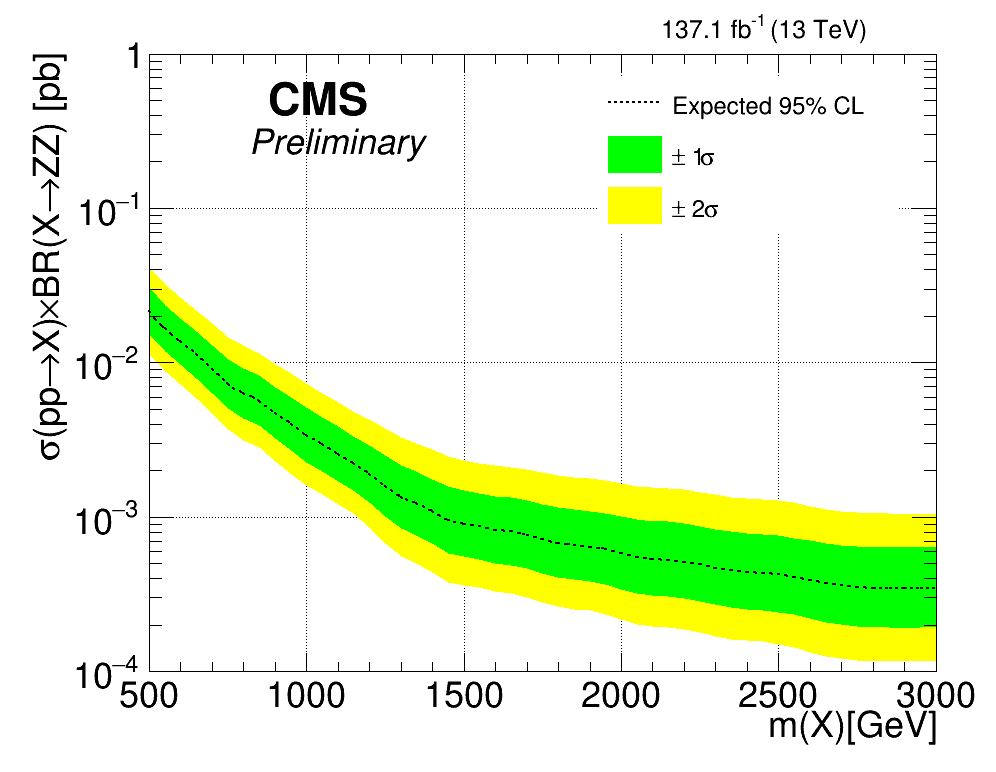
\includegraphics[width=\textwidth]{figures/HighMassSearches/Limit/highMassLimit_spin0_2D_13TeV_run2__run2_22may_blind_.png}
 }
 \caption{
 Expected upper limits on the $pp\to {\rm X}\to  {\rm ZZ}$ cross section
 %for 36.9 $fb^{-1}$
 of CMS data at 13 TeV where the fraction of VBF production is allowed to float in the fit.
 \label{fig:highmassresult}}
 \end{figure}
 %%%%%%%%%%%%%%%%%%%%%%%%%%%%%%

 \section{Summary}
 \label{sec:Summary}

  A search for a new scalar resonance decaying to a pair of $\cPZ$ bosons is performed for a range of masses
 between 500\GeV and 3\TeV with the full data set recorded by the CMS experiment at 13\TeV during 2016 - 2018
 and corresponding to an integrated luminosity of \usedLumi.


